\documentclass[10pt,border=4pt]{standalone}
\usepackage{mathptmx}
\usepackage{amsmath,amssymb,bm}
\usepackage{tikz}
\usetikzlibrary{patterns,decorations.pathmorphing,decorations.pathreplacing,arrows.meta,fit,backgrounds,calc,positioning,shapes.geometric}
\definecolor{acc}{HTML}{0B5394}
\definecolor{accl}{HTML}{EAF0F7}
\definecolor{grp}{HTML}{F5F5F5}
\definecolor{org}{HTML}{C55A11}
\definecolor{orgl}{HTML}{FBEFE6}
\tikzset{
 dat/.style={draw=black,line width=0.6pt,fill=white,align=center,font=\small,inner sep=3pt,minimum height=0.85cm},
 lay/.style={draw=acc,line width=0.8pt,fill=accl,rounded corners=2pt,align=center,font=\small,inner sep=3pt,minimum height=0.85cm},
 cnd/.style={draw=org,line width=0.8pt,fill=orgl,rounded corners=2pt,align=center,font=\small,inner sep=3pt,minimum height=0.75cm},
 op/.style={circle,draw=black,line width=0.6pt,fill=white,inner sep=0.5pt,font=\small,minimum size=5mm},
 grpb/.style={draw=black!45,dashed,line width=0.6pt,rounded corners=3pt,inner sep=6pt},
 arr/.style={-{Latex[length=2.2mm,width=1.7mm]},line width=0.7pt},
 carr/.style={-{Latex[length=2.2mm,width=1.7mm]},line width=0.7pt,draw=org},
 shp/.style={font=\scriptsize,text=black!70,inner sep=1pt},
 lab/.style={font=\footnotesize,inner sep=1pt},
 ttl/.style={font=\small\bfseries,inner sep=0pt,anchor=west}
}
\newcommand{\xh}{\mathbf{x}_h}\newcommand{\xf}{\mathbf{x}_f}

\tikzset{dim/.style={{Latex[length=1.5mm]}-{Latex[length=1.5mm]},line width=0.5pt}}
\begin{document}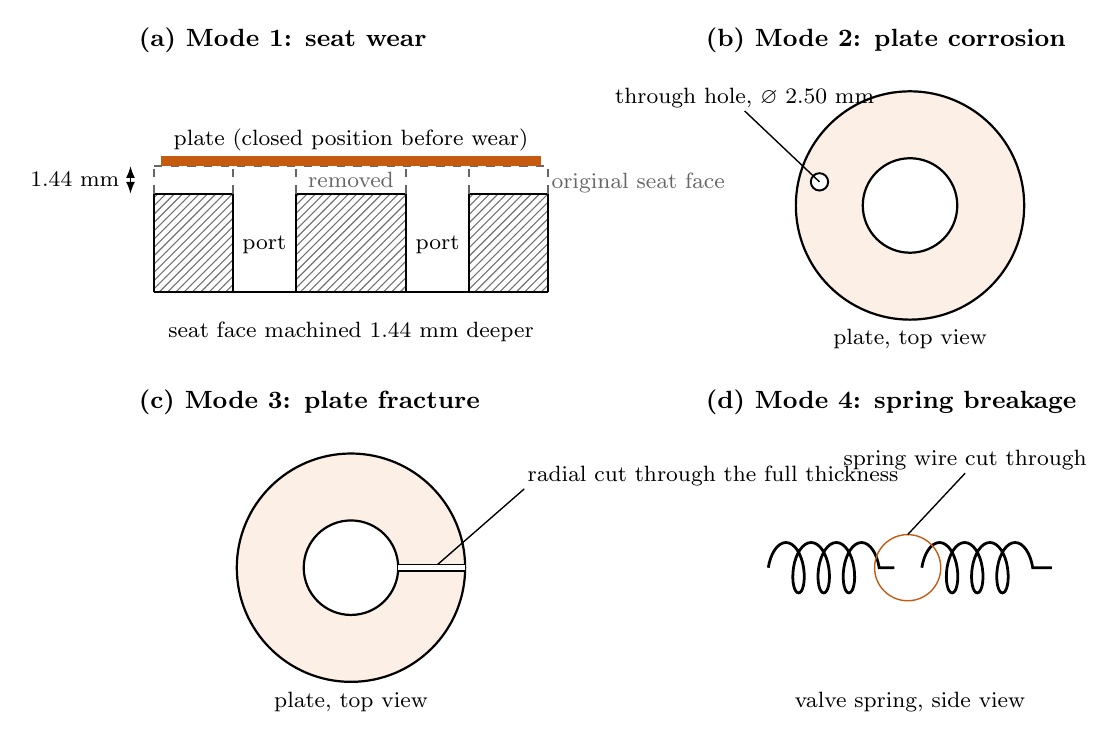
\begin{tikzpicture}[x=1cm,y=1cm]
% (a) seat wear: section of the seat
\node[ttl] at (0,3.2) {(a) Mode 1: seat wear};
\fill[pattern=north east lines,pattern color=black!55] (0.2,0) rectangle (1.2,1.6) (2.0,0) rectangle (3.4,1.6) (4.2,0) rectangle (5.2,1.6);
\fill[white] (0.2,1.25) rectangle (5.2,1.62);
\draw[line width=0.8pt] (0.2,0)--(0.2,1.25)--(1.2,1.25)--(1.2,0) (2.0,0)--(2.0,1.25)--(3.4,1.25)--(3.4,0) (4.2,0)--(4.2,1.25)--(5.2,1.25)--(5.2,0) (0.2,0)--(5.2,0);
\draw[dashed,line width=0.7pt,black!60] (0.2,1.6)--(5.2,1.6) node[lab,right,yshift=-6pt]{original seat face};
\draw[line width=0.8pt,draw=org,fill=org] (0.3,1.62) rectangle (5.1,1.72);
\node[lab,anchor=south] at (2.7,1.75) {plate (closed position before wear)};
\draw[dim] (-0.1,1.25)--(-0.1,1.6); \node[lab,anchor=east] at (-0.2,1.43) {1.44 mm};
\draw[dashed,line width=0.5pt,black!60] (0.2,1.25)--(0.2,1.6) (1.2,1.25)--(1.2,1.6) (2.0,1.25)--(2.0,1.6) (3.4,1.25)--(3.4,1.6) (4.2,1.25)--(4.2,1.6) (5.2,1.25)--(5.2,1.6);
\node[lab,black!60] at (2.7,1.43) {removed};
\node[lab] at (1.6,0.6) {port}; \node[lab] at (3.8,0.6) {port};
\node[lab,align=center] at (2.7,-0.5) {seat face machined 1.44 mm deeper};
% (b) plate corrosion
\begin{scope}[shift={(8.6,0)}]
\node[ttl] at (-1.4,3.2) {(b) Mode 2: plate corrosion};
\draw[line width=0.8pt,fill=orgl,even odd rule] (1.2,1.1) circle (1.45) (1.2,1.1) circle (0.6);
\fill[white,draw=black,line width=0.7pt] (0.05,1.4) circle (0.11);
\draw[line width=0.5pt] (0.05,1.4)--(-0.9,2.3) node[lab,anchor=south]{through hole, $\varnothing$ 2.50 mm};
\node[lab] at (1.2,-0.6) {plate, top view};
\end{scope}
% (c) plate fracture
\begin{scope}[shift={(0,-4.6)}]
\node[ttl] at (0,3.2) {(c) Mode 3: plate fracture};
\draw[line width=0.8pt,fill=orgl,even odd rule] (2.7,1.1) circle (1.45) (2.7,1.1) circle (0.6);
\draw[line width=1.6pt,white] (3.3,1.1)--(4.15,1.1); \draw[line width=0.5pt] (3.3,1.06)--(4.15,1.06) (3.3,1.14)--(4.15,1.14);
\draw[line width=0.5pt] (3.8,1.14)--(4.9,2.1) node[lab,anchor=south west]{radial cut through the full thickness};
\node[lab] at (2.7,-0.6) {plate, top view};
\end{scope}
% (d) spring breakage
\begin{scope}[shift={(8.6,-4.6)}]
\node[ttl] at (-1.4,3.2) {(d) Mode 4: spring breakage};
\draw[line width=1.0pt,decorate,decoration={coil,aspect=0.45,segment length=3.2mm,amplitude=3.2mm}] (-0.6,1.1)--(1.0,1.1);
\draw[line width=1.0pt,decorate,decoration={coil,aspect=0.45,segment length=3.2mm,amplitude=3.2mm}] (1.35,1.1)--(3.0,1.1);
\draw[line width=0.5pt,draw=org] (1.17,1.1) circle (0.42);
\draw[line width=0.5pt] (1.17,1.52)--(1.9,2.3) node[lab,anchor=south]{spring wire cut through};
\node[lab] at (1.2,-0.6) {valve spring, side view};
\end{scope}
\end{tikzpicture}\end{document}
